\section{Brukergrensesnitt \texttt{(View)}} \label{sec:brukergrensesnitt}

\subsection{Oppstart av brukergrensesnittet}
I \texttt{MainController.java} instansieres først to Arkfaner, \texttt{ArkfaneMegler.java} og \texttt{ArkfaneAnnonse.java}.
Disse sendes så med som parametere inn i strukturen til brukergrensesnittet, først til \texttt{StartGUI.java}, og så videre til \texttt{MainPanel.java} som oppretter \texttt{JTabbedPane} og legger inn de to arkfanene der.
Grunnen til at arkfanene ble opprettet allerede i \texttt{MainController.java} er fordi vi sender med det respektive arkfane under instansiering av \texttt{Kontrollerne}. 
Siden de to arkfanene har så lik funksjonalitet, deler de på \texttt{Kontrollerne} som de har felles.

Fra \texttt{MainController.java} opprettes det to versjoner av \texttt{ControllerTabell.java}. Til den ene sendes vinduet \texttt{meglerVindu} som er instans av \texttt{ArkfaneMegler.java} og til den andre kontrollerinstansen sendes \texttt{annonseVindu} som er instans av \texttt{ArkfaneAnnonse.java}.
Se illustrasjonen nedenfor.
\begin{figure}[ht]
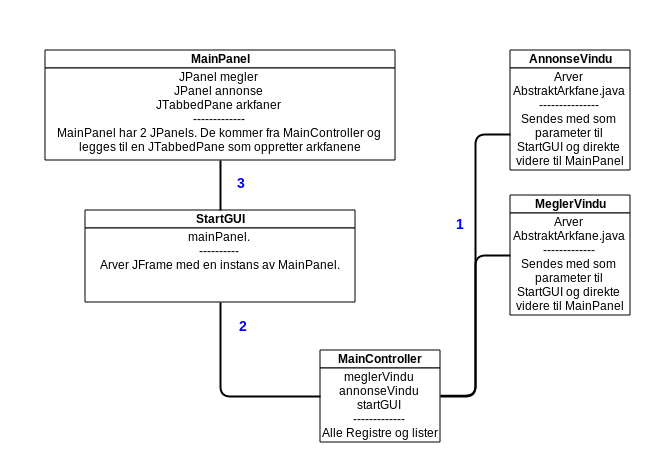
\includegraphics[width=\textwidth,height=\textheight,keepaspectratio]{./img/produktdokumentasjon/bilder/Controller_og_GUI-opprettelse2.png}
\caption{Illustrasjon over hvordan \texttt{MainController} starter opp programmet}
\end{figure}

\subsection{Bruk av arv i brukergrensesnittet}
Brukergrensesnitt er utrolig tidkrevende å jobbe med, og veldig mye av det man gjør er å skrive samme kode for hvert enkelt vindu.
For å unngå dette mest mulig, samt å få alle vinduer og paneler til å ha mest mulig den samme følelsen har vi noen abstrakte klasser som vi arver på tvers av alle klassene som har med brukergrensesnitt å gjøre.

\subsubsection*{\texttt{AbstractPanel.java}}
Dette panelet arver \texttt{JPanel} og er superklassen til alle andre hovedvinduer og paneler i programmet.
Denne klassen har to \texttt{konstruktører}. Den ene tar inn to heltall som representerer bredde og høyde på det panelet som arver klassen, samt en \texttt{String borderTitle} som blir tittel på kantlinjen som \texttt{konstruktøren} oppretter.
Den andre \texttt{konstruktøren} er omtrent lik, men tar ikke inn en \texttt{String} for kantlinje, så her kan man velge mellom to \texttt{konstruktører}, med eller uten kantlinje.
Dette panelet er også satt med en bakgrunnsfarge slik at alle paneler og vinduer som arver denne vil arve denne.

\texttt{CustomSubPanel.java} arver også \texttt{AbstractPanel.java}. Denne klassen brukes i hovedsak for paneler inne i et hovedpanel. Da dette panelet skal brukes gjentatte ganger i mange forskjellige sammenhenger er det hele 6 \texttt{konstruktører} her. 
I noen opprettes det en predefinert \texttt{Layout}, i andre ikke. Noen tar inn størrelse (bredde og høyde), andre ikke. På denne måten har vi fått en veldig slagkraftig klasse som har spart oss for mye arbeid og forenklet konstruksjonen av brukergrensesnitter veldig.

\subsubsection*{\texttt{AbstractRegistreringsVindu.java} og \texttt{AbstractRegistreringsPanel.java}}
\texttt{AbstractRegistreringsVindu.java} er superklassen for \texttt{AbstractRegistreringsPanel.java}. Denne klassen arver \texttt{JFrame} og er setter de mest generelle parameterne som et hvert vindu skal ha. Størrelse, navn på vinduet, samt standard lukkefunksjonalitet osv.
\texttt{AbstractRegistreringsPanel.java} er superklassen til alle registreringsvinduene. Denne klassen har en \texttt{BorderLayout} og tar inn parametere som bredde, høyde og tittel for vinduet som opprettes. Ut over dette gjør ikke denne klassen mye. Alle klasser som arver denne vil velge hvilke paneler fra denne klassens \texttt{BorderLayout} de ønsker å ta i bruk.

\subsection{Oppbyggningen av arkfanene}
Begge arkfanene er bygget over samme lest. De arver \texttt{AbstraktArkfane.java}. Denne klassen tar inn en \texttt{String} som avgjør hvilke \texttt{topPanel} som skal følge med arkfanen.
\texttt{AbstraktArkfane.java} består i korte trekk av en \texttt{BorderLayout} med fire paneler; \texttt{toppanel, venstrepanel, senterpanel} og \texttt{bunnpanel}.
Hvert av panelene er satt opp med en \texttt{get-metode} som brukes hyppig av \texttt{kontrollerne} i kommunikasjonen med komponentene der.

Alle \texttt{kontrollerne} er "klar" over sitt vindu, og nedenfor er et eksempel på hvordan \texttt{ControllerTabell.java} kommuniserer med vinduet.

\begin{lstlisting}[caption=Kodeeksempel på hvordan \texttt{ControllerTabell.java} kommuniserer med brukergrensesnittet]
        /**
         * Lytter på museklikk i Output-vinduet.
         */
        vindu.getSenterpanel().getEditorPane().addMouseListener(new MouseAdapter() {

            @Override
            public void mouseClicked(MouseEvent e) {
                if (e.getButton() == MouseEvent.BUTTON1) {
                    if (modellIBruk instanceof TabellModellAnnonse) {
                        Annonse valgtObjekt = returnerAnnonseObjekt();
                        if (vindu instanceof ArkfaneMegler) {
                            new ControllerBildeViser(valgtObjekt.getBolig(), true);
                        } else {
                            new ControllerBildeViser(valgtObjekt.getBolig(), false);
                        }
                    }
                }
            }

        });
\end{lstlisting}

